

Before I dive into the details of C++20, I want to give a quick overview of the features in C++20.
This overview should serve two purposes; to give a first impression, and to provide links to the relevant sections you can use to dive directly into the details. Consequently, this chapter has only code snippets, but no complete programs.

My book starts with a short historical detour into the previous C++ standards. This detour provides context when comparing C++20 to previous revisions and demonstrates the importance of C++20 by providing a historical context.

\begin{center}
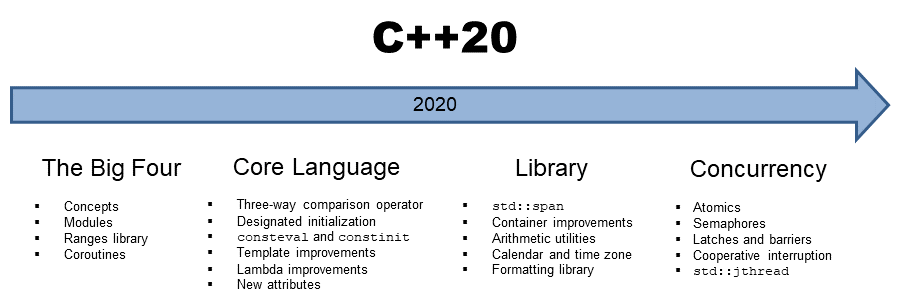
\includegraphics[width=1.0\textwidth]{content/2/chapter3/images/1.png}\\
\end{center}

C++20 has four outstanding features: concepts, ranges, coroutines, and modules. Each deserves its own subsection.








